\section{Computer Setup}
\begin{information}
We will all be working on our own computers today, and will be accessing Virtual Machines running the Ubuntu operating system on the Nectar Research Cloud (\url{http://nectar.org.au/}).
The software client No Machine which you will have already installed, enables us to access these machines in a familiar Desktop style, even though the majority of our time will be spent within the terminal. \\
\end{information}

\begin{warning}
If you did not install NoMachine prior to today's workshop, the correct installers can be found at:
\begin{itemize}
	\item \url{http://tinyurl.com/lcn3ns8} (Windows)
	\item \url{http://tinyurl.com/mnm23ew} (Mac)
\end{itemize}
\end{warning}

\begin{information}
No Machine session files will be provided to each attendee which have been pre-configured to enable easy access to these machines.
These machines are effectively dual-core machine with 8GB of RAM \& 70GB of hard drive space.
Whilst relatively small, this will be more than enough to become familiar with the important concepts for the day.
To begin today's session, simply click (or double-click) on the No Machine session file that you have been given.
The desktop from the Virtual Machine (VM) that you have connected to will appear on the
No Machine client. \\
\end{information}

\begin{figure}[h!]
  \centering
    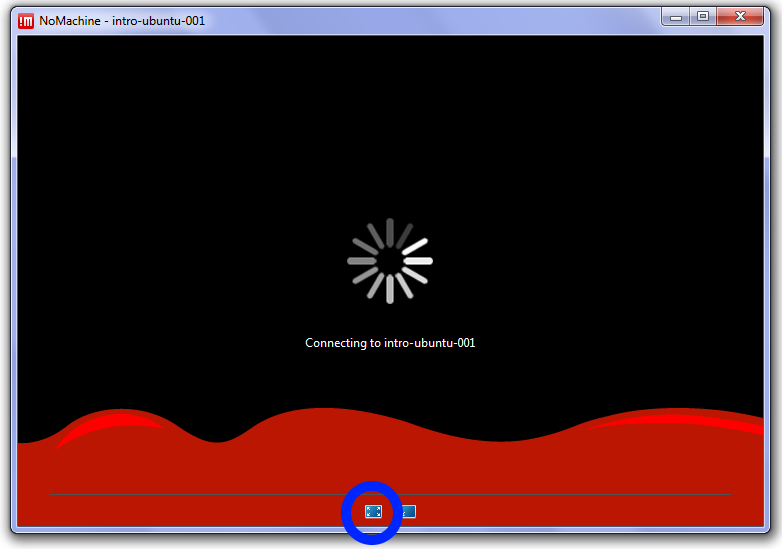
\includegraphics[width=0.8\textwidth]{images/NoMachine.png}
\end{figure}

\begin{warning}
While this is connecting, select the button circled in blue above.
This will resize NoMachine to be full screen to feel more like you are physically located at the VM.
If any security warnings appear, ignore them \& continue connecting.
This may take several attempts and if you can't connect after 3 or 4 times, call a tutor over.
\end{warning}

If you forgot to set the client to full screen, hover your mouse over the top-right corner and click where the `page' folds over. 
This will enable you to resize the client again, and can also be used to disconnect from the VM.\\


\section{The Ubuntu Desktop}
\begin{note}
Now that you are connected, you will notice we are in a standard graphical environment.
The default Desktop in Ubuntu is Unity, but what we are seeing is known as the Gnome Desktop, as is the default for Nectar VMs.
As many of us are used to seeing, there are click-able icons on the desktop, and drop-down menus. \\

The main interfaces we will be using today are the \texttt{terminal}, a text editor named \texttt{gedit} and the web browser \texttt{firefox}
They will appear as icons on the desktop, but can also be accessed from the drop-down menus.
A \texttt{Firefox} icon is also located on the desktop \& this can be used for searching for answers as well as viewing the output of \texttt{fastqc}.
%When viewing clips  you will be unable to obtain sound from the VM, so switch back to your normal laptop for these.
\end{note}

\subsection{Basic Shell Comands}
\begin{note}
Today we will assume a basic familiarity with the bash terminal in Linux.
Some key commands which we will be using are explained in the following table.
\end{note}
\begin{center}
  \begin{tabular}[h]{|p{3cm} | p{11.5cm} |}
    \hline
    \textbf{Command} & \textbf{Meaning} \\
    \hline
    \texttt{cd} & Change directory \\
    \texttt{ls} & List files in a directory \\
    \texttt{man} & Call the manual for a given command \\
    \texttt{head} & View the first 10 lines of a file \\
    \hline
  \end{tabular}
\end{center}

\begin{steps}
Open a terminal in the VM by either clicking on the icon, or using the drop-down menu.
It will automatically open in your home directory (\texttt{/home/trainee}), which is indicated by the tilde before the dollar sign.
The tilde (\~{}) is a symbolic representation of the address \texttt{/home/trainee}, where the first slash is the root of the computer’s file system.
To return to this directory from any other in the file system, you can simply enter the command
\begin{lstlisting}
cd 
\end{lstlisting}
\end{steps}

Normally we specify the directory to change into after the command \texttt{cd}, but when no directory is given, this command will automatically change to your home directory.\\

\begin{warning}
Please note, the Linux operating system is case-sensitive.
When entering the any commands, please make sure that you pay attention to this detail.
Spaces are an important feature as well, so be careful not to add or omit them where they appear in any sample code.
\end{warning}

\section{Today's Data}

\begin{information}
Before we begin today's session, we need to download and run a script.
This will make all the correct directories on your VM and download the data for today's session.
\end{information}

\begin{steps}
The script can be obtained from \url{http://tinyurl.com/hkc77vf}.
Head to this address using \texttt{firefox} and save this on your VM as the script \texttt{getNGSData.sh}.
It won't matter where, but \texttt{firefox} will probably place it in your \texttt{Downloads} directory.\\

Now open a terminal and head to the folder the file was saved in.
The following assumes that the file was saved in your \texttt{Downloads} directory.
\begin{lstlisting}
cd ~/Downloads
chmod +x getNGSData.sh
./getNGSData.sh
\end{lstlisting}
\end{steps}

This will start downloading all of the files to your VM and will create a directory \texttt{/home/trainee/NGSData} with today's data.

\begin{advanced}
If you're curious open the script we've just run using gedit and see if you can understand what the script has done.
You might be surprised at how much you understand.
\begin{lstlisting}
gedit getNgsData.sh &
\end{lstlisting}
\end{advanced}

\subsubsection*{Today's Notes}
Today's notes are also available electronically from the site \url{http://uofabioinformaticshub.github.io/Intro-NGS\_2016-03-31/}